\headline{{\textbf{\Large\sffamily Special Report: The Engine Room}}\\
{\textbf{\large\sffamily A Deep Dive into Bonsai Horticulture\\ with Andy Hardman}}}
\phantomsection
\label{2026-01-hardman-report}

\noindent
During the quiet months of the pandemic, our club was privileged to host a deep-dive virtual workshop with \textbf{Andy Hardman}.
For those who missed it---or those whose notes have gathered dust---this article reorganizes Andy's masterclass on the horticultural ``engine'' of bonsai: the substrate and the nutrients we fuel it with.

As we approach the repotting season, we have also synthesized this with the \textbf{TWBC New \& Existing Members Information Pack} (available in full on our Discord channel) to provide a comprehensive guide for every bench in the club.

\topic{Introduction \& The Goal of Bonsai Horticulture}
\noindent
Andy Hardman's approach to bonsai is rooted in a fundamental shift of perspective: we do not grow trees; we grow roots.
The rest of the tree is simply a byproduct of the health of the root system.
In this workshop, Andy challenges the ``traditional'' recipes often found in older books, urging members to look at the specific physiological needs of a tree living in the highly artificial environment of a ceramic pot.
The ultimate goal is to achieve the most efficient root growth possible, ensuring that every cubic centimetre of the container is working toward the tree's health.

\topic{Root Physiology: The Real Engine}
\noindent
To master soil, we must first master the biology of the root.
Andy makes a critical distinction between the woody roots we see and the microscopic \textbf{root hairs} that do the actual work.
These hairs have a very short lifespan and are responsible for the entire uptake of water and nutrients.

\textit{``They don't grow in space; they grow on surfaces,''} Andy notes.
Therefore, the more surface area our soil provides, the more ``engine'' we can build.
He also warns of the ``fear factor'' of repotting: when we bare\--root or aggressively clean a tree, we are effectively ripping off the tree's mouth.
Understanding this vulnerability is key to deciding which substrate to use for a fast recovery.

\topic{The Physical Requirements of a Substrate}
\noindent
A successful substrate must manage the delicate balance between oxygen and water.
The primary obstacle to this is \textbf{Surface Tension}.
When soil particles are too fine, water creates a physical seal across the gaps, preventing gas exchange.

Andy's solution is the ``Two-Millimetre Rule.'' By ensuring that:

\vspace*{-0.751em}
$$ \text{Particle Size} \geq 2 \text{mm} $$

\noindent
we break the surface tension of water.
This allows the pot to drain freely, pulling oxygen into the core of the root ball.
Furthermore, he addresses the ``Freeze-Thaw'' cycle.
Since water expands by roughly 9\% when it freezes:

\vspace*{-0.75em}
$$ \text{Vice} \approx 1.09 \times V_\text{water} $$

\noindent
soft substrates like Akadama can be physically crushed into dust in a single hard winter, leading to the exact compaction and suffocation we try to avoid.

\topic{Chemical and Surface Properties}
\noindent
Beyond physics, we look at \textbf{Cationic Exchange Capacity (CEC)}.
This is the soil's ability to ``hold'' nutrients electrically.
Without CEC, your fertilizer is simply washed out of the drainage holes.
Andy also stresses the importance of \textbf{Surface Texture}.
Rough, jagged volcanic particles like lava and pumice are superior to smooth grit because they physically force root tips to split (ramify) upon contact, creating the fine, fibrous network we desire.

\topic{Soil Report Card}
\noindent
Andy provides a candid breakdown of modern materials:

\begin{itemize}
    \item \textbf{Pumice & Lava:} The resilient ``all\--rounders.''
    They are porous, frost-proof, and offer excellent surface texture.

    \item \textbf{Akadama:} Unrivalled for CEC and moisture control, but its ``softness'' makes it a liability in wetter, colder UK winters unless protected.

    \item \textbf{Horticultural Grit:} Famously dismissed by Andy as \textbf{``wasted space.''}
    It has 0\% CEC and 0\% porosity.

    \item \textbf{Cat Litter:} A viable budget\--friendly molar clay, but often lacks the jagged texture of volcanic rock.
\end{itemize}

\topic{Nutrient Science: N-P-K}
\noindent
Fertilizing is the fuel for the engine.
We must understand the ``Big Three'':

\begin{itemize}
    \item \textbf{Nitrogen (N):} For green mass and chlorophyll production.

    \item \textbf{Phosphorus (P):} For root strength and flowering.

    \item \textbf{Potassium (K):} For disease resistance and internal transport.
\end{itemize}

Andy clarifies a common myth: adding more liquid fertilizer to a pot doesn't help if the water is already saturated.
To give a tree more food, you must increase the \textit{percentage} (the numbers on the bottle), not just the frequency.

\topic{The Seasonal Feeding Regime}
\noindent
The tree's needs change with the sun.
\textbf{Spring} requires a Nitrogen\--heavy approach (e.g., 10:6:6) to trigger growth.
By \textbf{Summer}, we move to a balanced 7:7:7.
As we enter \textbf{Autumn}, we reduce Nitrogen to near zero, increasing Phosphorus and Potassium (e.g., 3:10:10) to ``harden off'' the wood and prepare the buds for next year.
Importantly, Andy advises that feeding should stop entirely when temperatures drop below $8^\circ\text{C}$, as the tree's metabolic processes simply cannot process it.

\topic{Organic vs. Chemical Fertilizers}
\noindent
The presentation concludes with a strong recommendation for \textbf{Organic Fertilizers}.
Chemical salts act fast but can be ``hot'' and destroy the delicate \textbf{Micro\--culture} of the soil.
Organics (Bio\--Gold, Naruko, Green Dream) require soil bacteria to break them down, ensuring a slow, safe release of nutrients.
Andy also advocates for the use of ``biostimulants'' like \textbf{Seaweed} and \textbf{Fish Emulsion}, which don't just feed the tree, but feed the soil organisms that keep the tree healthy.
\vfill
\closearticle

\clearpage


%\headline{{\textbf{\Large\sffamily Rooted in Success:}}\\
%          {\textbf{\large\sffamily A Masterclass in Soil and Nutrition}}}
%\label{2025-12-workshop-mep}
%
%During the quiet months of the pandemic, our club was privileged to host a deep-dive virtual workshop with \textbf{Andy Hardman}.
%For those who missed it—or those whose notes have gathered dust—this article reorganizes Andy's masterclass on the horticultural ``engine'' of bonsai: the substrate and the nutrients we fuel it with.
%
%As we approach the repotting season, we have also synthesized this with the \textbf{TWBC New \& Existing Members Information Pack} (available in full on our Discord channel) to provide a comprehensive guide for every bench in the club.
%
%
%
%%\topic{The Birth of a New Tradition}
%%\noindent
%%Following the initial proposal back in August, the Member Education Programme (MEP) has officially transitioned from a promising concept to a vibrant reality. The initiative was born out of a desire to bridge the gap between watching demonstrations and hands-on practice. The response from the membership was immediate and overwhelming, with 19 members voting in favour of the launch. This enthusiasm has translated directly into bookings; since opening the registrations, seats for the scheduled sessions have been snapped up almost instantly, proving that there is a significant appetite within the Twickenham Bonsai Club for structured, mentor-led learning.
%%
%%The MEP is designed specifically to support our novice members by pairing them with more experienced practitioners. By providing a dedicated space and time, the club ensures that the "Twickenham family" spirit continues to thrive, passing down years of collective wisdom in a focused environment.
%%
%%\medskip
%%\topic{A Saturday Morning at Whitton}
%%\noindent
%%On Saturday, 13th December, the Whitton Community Centre's front room was transformed into a bustling bonsai studio for our inaugural session. Transitioning from our usual Thursday evening meetings to a Saturday morning proved to be a masterstroke of convenience. Avoiding the post-work rush allowed for a refreshed start, and the atmosphere was noticeably different—relaxed, yet buzzing with intent.
%%
%%Upon arrival, I found the space perfectly organised. Large tables were set up, providing ample room for each participant to spread out their tools and trees. The theme for the morning was \textbf{winter structural pruning and wiring}. Tony Ulatowski and Chris Durne led the session, moving methodically between the tables. Their approach was particularly commendable: they began by listening. Each participant had the opportunity to explain their tree's history and their goals before receiving a tailored array of advice.
%%
%%The technical guidance was profound. We moved beyond simple aesthetics, diving deep into the physiology of the trees. Suggestions ranged from bold structural choices—removing major branches to improve the silhouette—to advanced techniques like double-wiring trunks for heavy bends or using guy wires to set long-term development. Senior members, including Terry and Tina, worked on their own trees while simultaneously offering a helping hand to others, creating a seamless flow of mentorship.
%%
%%\medskip
%%\topic{Personal Reflections: More Than Just Pruning}
%%\noindent
%%As I worked on my own trees, I felt a genuine shift in my understanding of the craft. It wasn't just about where to cut, but why. The "fear factor" that often haunts novice growers began to dissipate, replaced by a sense of calculated confidence. I managed to bring along my dog, who would have otherwise spent the morning howling at home—a small but significant detail that highlights the welcoming, community-oriented nature of these Saturday sessions.
%%
%%In my view, the MEP represents the very best of TWBC. It is an investment in the members themselves. By covering the venue costs, the club has removed the barriers to entry, allowing us to focus entirely on the art. I left the session feeling that I had made more progress in three hours than I might have in months of solitary practice.
%%
%%\end{multicols}
%%\vspace*{2em}
%%\begin{minipage}[b]{1.0\textwidth}
%%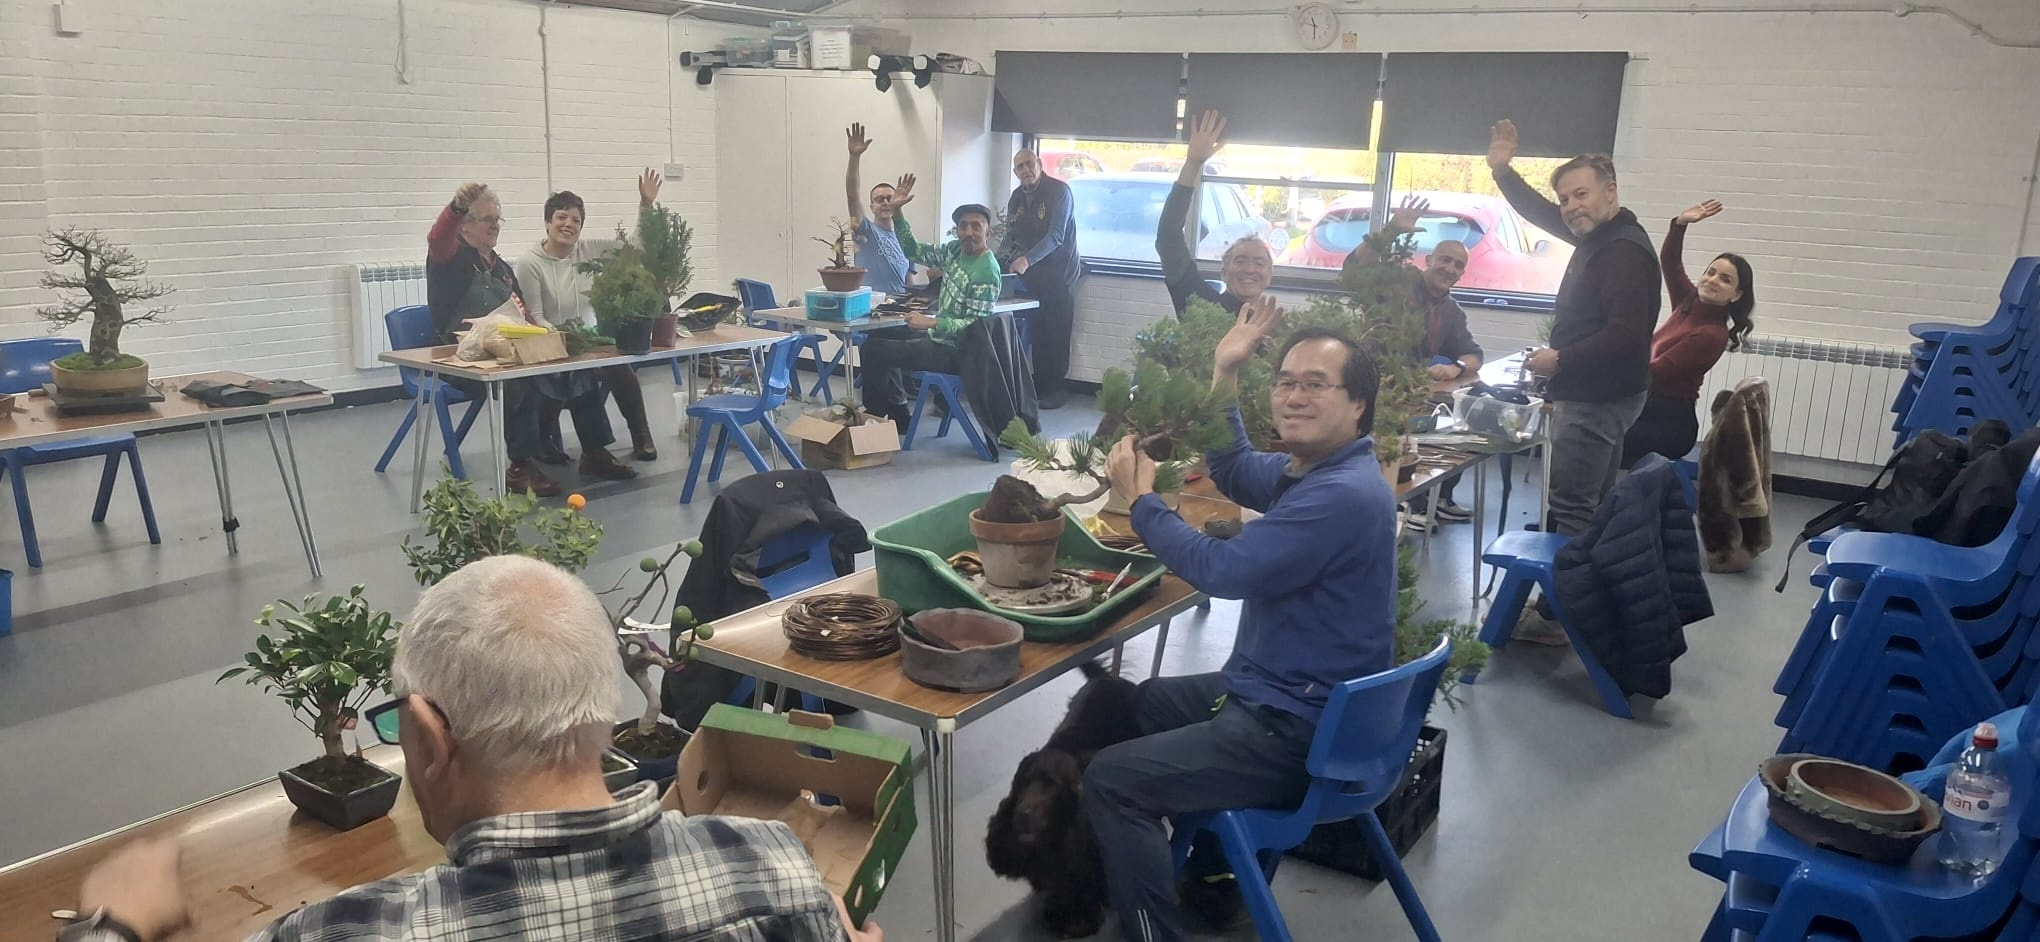
\includegraphics[angle=0,origin=c,width=1.0\textwidth]{2025_12/res/workshop-mep-opening}
%%\centerline{\emph{The buzzing atmosphere and camaraderie during TWBC's first MEP workshop.}}
%%\end{minipage}
%%\medskip
%%\begin{multicols}{2}
%%
%%\begin{minipage}[b]{0.45\textwidth}
%%\includegraphics[angle=0,origin=c,width=1.0\textwidth]{2025_12/res/workshop-mep-newsletters}
%%\centerline{\emph{Tony Ulatowski guiding a member on winter pruning.}}
%%\end{minipage}
%%
%%\begin{minipage}[b]{0.45\textwidth}
%%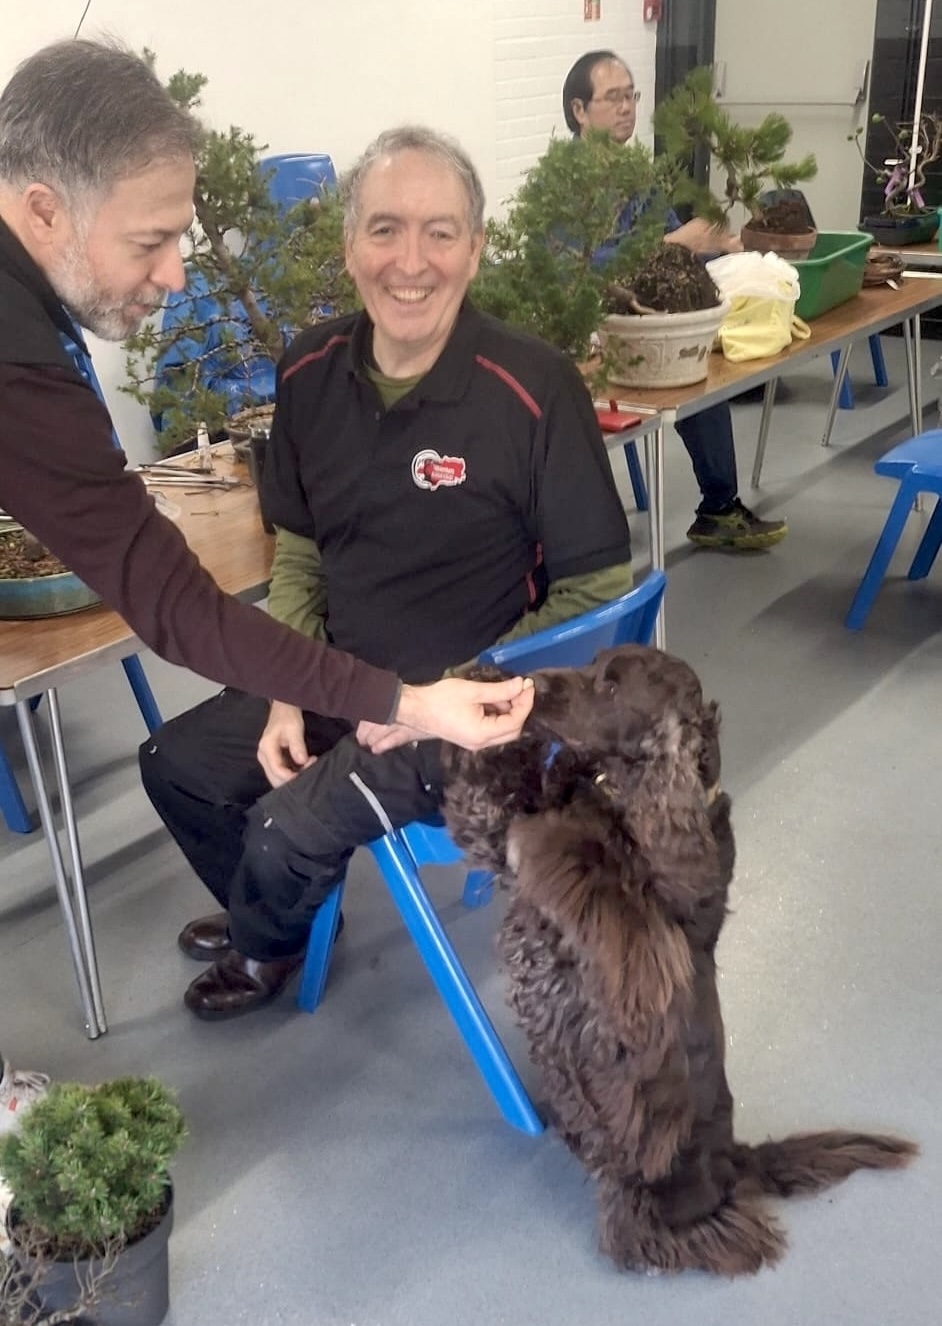
\includegraphics[angle=0,origin=c,width=1.0\textwidth]{2025_12/res/workshop-mep-durne}
%%\centerline{\emph{Chris Durne and a furry visitor enjoy the morning.}}
%%\end{minipage}
%%
%%\medskip
%%\topic{Voices from the Bench: Member Feedback}
%%\noindent
%%The sentiment across the room was echoed in the feedback received after the event. \textbf{John Mari} noted: \emph{"It's brilliant having guest speakers, but you can't beat working on your own trees and being guided by experts to really learn. I genuinely would love it to continue."}
%%
%%For many, the psychological boost was as important as the technical one. \textbf{Riz Mizra} shared: \emph{"Unlike other workshops, you don't feel silly asking weird questions. I got a great buzz from today!"} Similarly, \textbf{Martin Redfern} commented on the impact on his self-belief: \emph{"As someone who suffers with lack of confidence and vision, it really helped today to build a bit more positivity into my way of thinking about my abilities."} \textbf{Tina Todd} summed up the morning perfectly, asking: \emph{"Where did 3 hours go? I've gained a lot of confidence today."}
%%
%%\medskip
%%\topic{From the Organisers: A Positive Template}
%%\noindent
%%The organisers were equally encouraged by the turnout and the quality of work produced. \textbf{Chris Durne} remarked on the standard of the club: \emph{"No wonder TWBC is the best bonsai club in London with so many willing and able members."}
%%
%%\textbf{Tony Ulatowski} reflected on the broader mission of the programme: \emph{"The camaraderie in being together and sharing challenging feelings when working on trees is what we are about. We are putting members first in developing emotional confidence at all stages of the art. We now have a positive template in the MEP workshops."}
%%
%%\medskip
%%\topic{Looking Ahead: 2026 Sessions}
%%\noindent
%%Due to the incredible demand and the success of this first gathering, we are excited to look toward the next steps. The second scheduled session will take place on \textbf{Saturday, 17th January 2026}, focusing on \textbf{repotting and root pruning}.
%%
%%Because the January session filled up so quickly, Tony Ulatowski has kindly added an additional date to the calendar: \textbf{Saturday, 28th February 2026}. This extra session will also focus on repotting, specifically the critical art of positioning the tree within the container to achieve the best aesthetic balance. If you haven't secured a spot yet, please contact \textbf{Tony Ulatowski} or \textbf{Chris Durne} via WhatsApp immediately, as these final places are being snapped up fast.
%%
%%\medskip
%%\topic{Conclusion}
%%\noindent
%%The first MEP session was, by all accounts, a resounding success. It has strengthened our community, improved our trees, and most importantly, bolstered the confidence of our members. We owe a huge debt of gratitude to Tony, Chris, Terry, and Tina for their time and wisdom. The MEP has proven itself to be a vital new chapter for the Twickenham Bonsai Club, and I, for one, cannot wait for the next session.
%%
%%\closearticle
%%
%%\begin{minipage}[b]{0.45\textwidth}
%%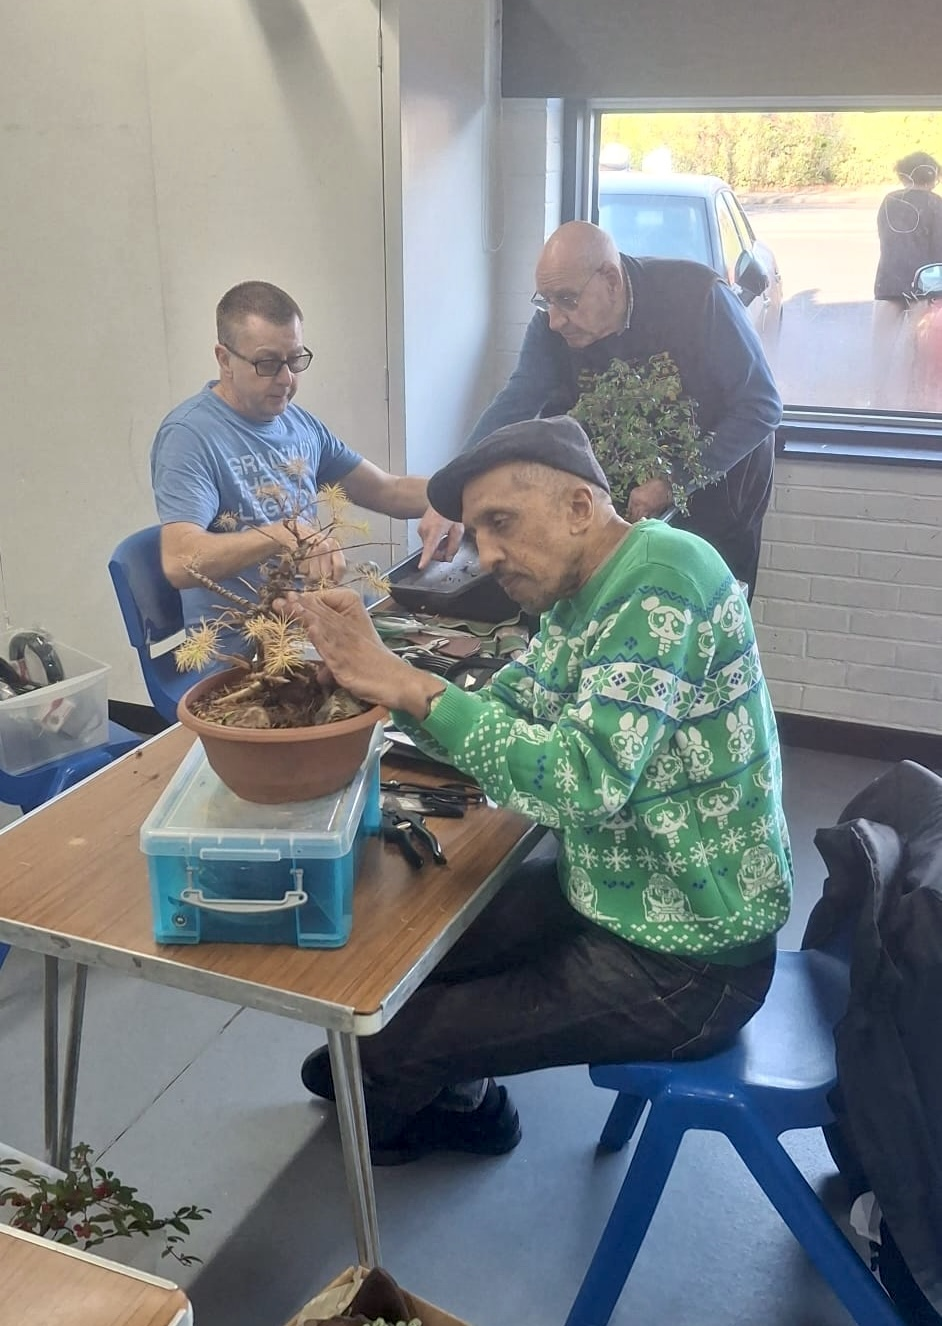
\includegraphics[angle=0,origin=c,width=1.0\textwidth]{2025_12/res/workshop-mep-wilson}
%%\centerline{\emph{Expert advice from Terry Wilson during the workshop.}}
%%\end{minipage}
%%
%%\begin{minipage}[b]{0.45\textwidth}
%%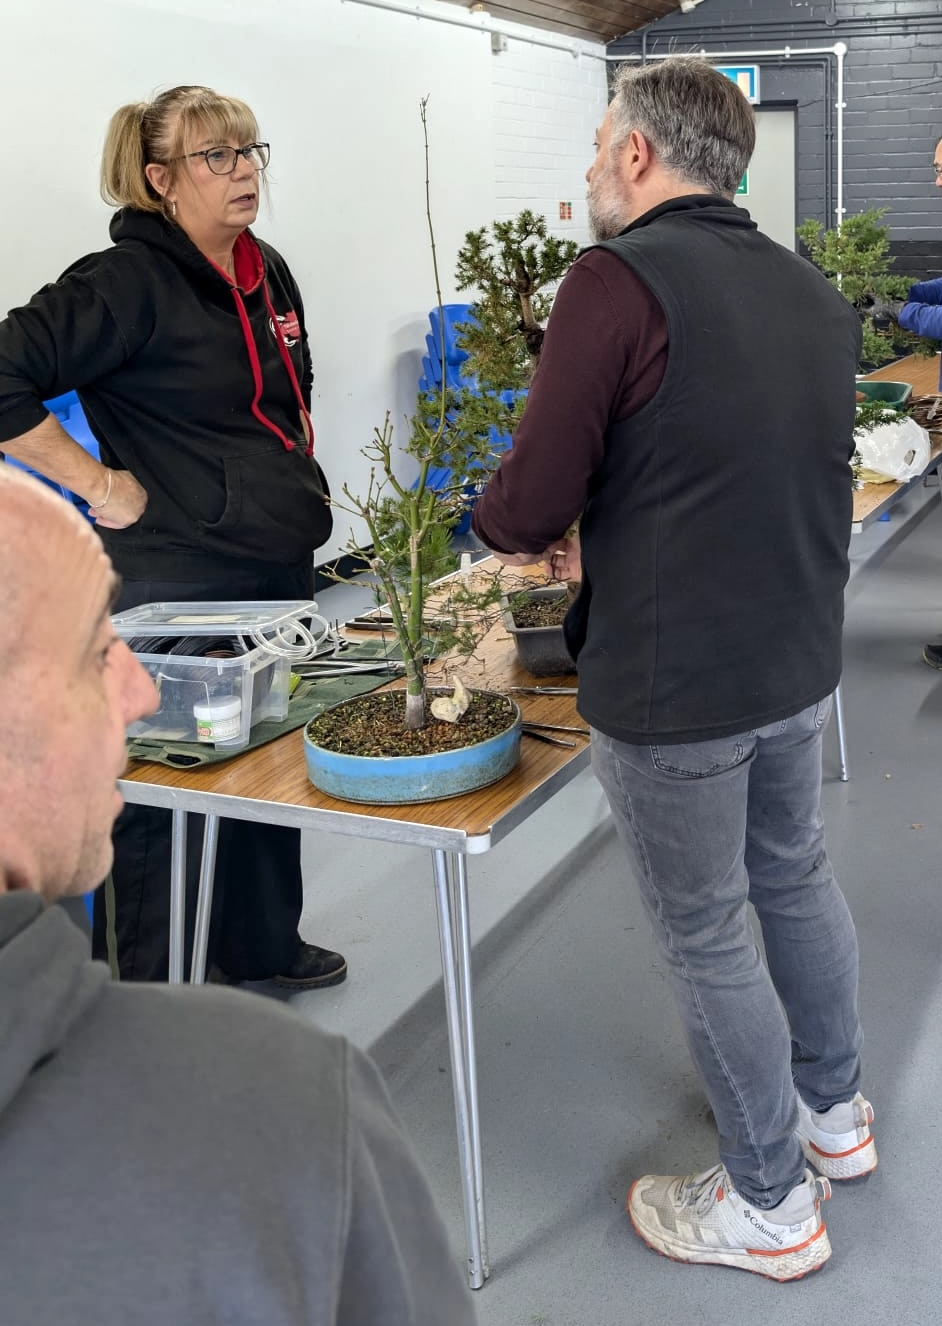
\includegraphics[angle=0,origin=c,width=1.0\textwidth]{2025_12/res/workshop-mep-todd}
%%\centerline{\emph{Tina Todd sharing her expertise with a fellow member.}}
%%\end{minipage}
%%
%%\begin{minipage}[b]{0.45\textwidth}
%%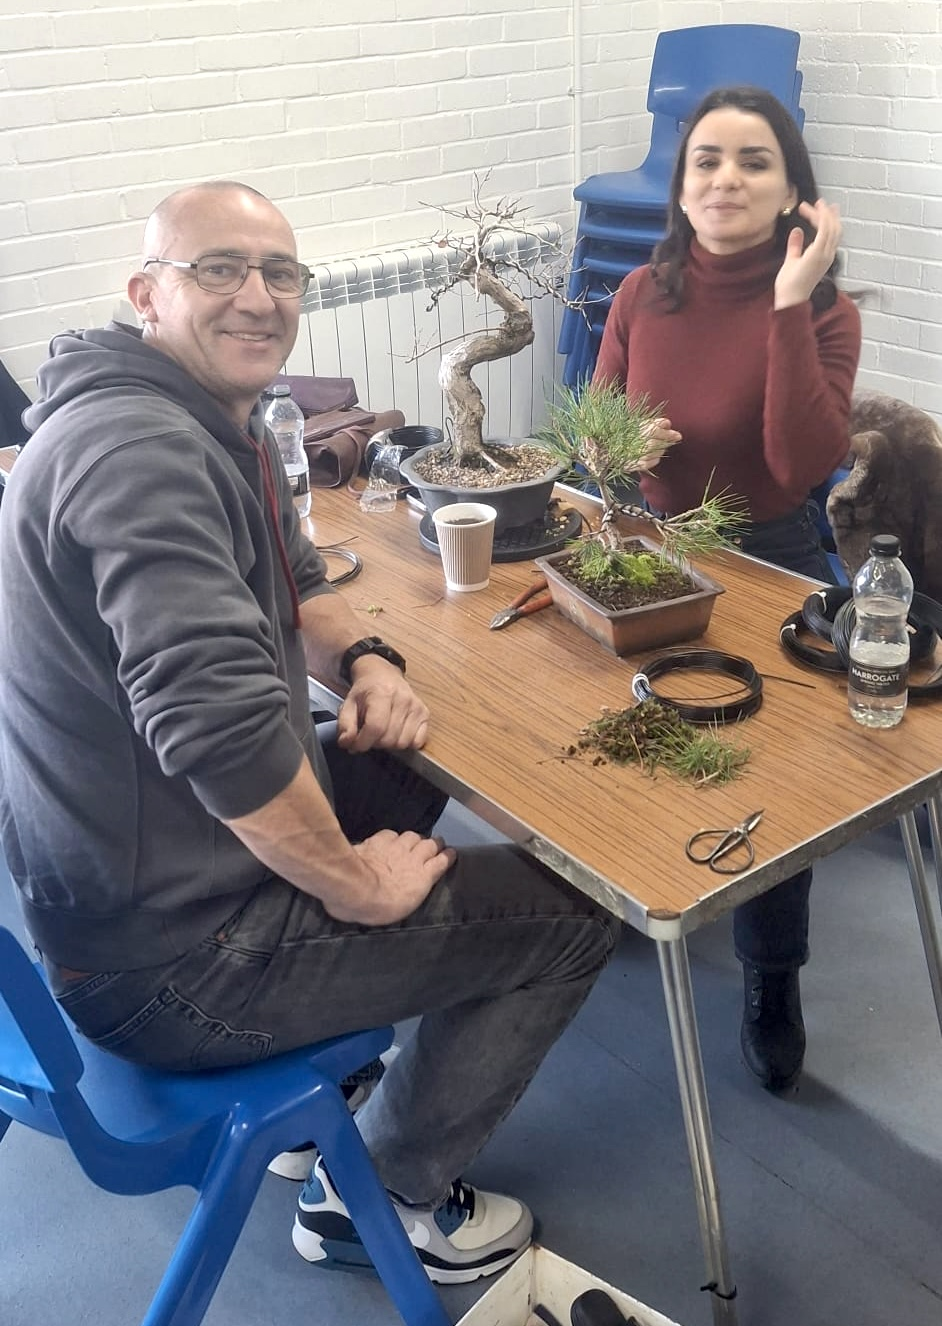
\includegraphics[angle=0,origin=c,width=1.0\textwidth]{2025_12/res/workshop-mep-members_1}
%%\centerline{\emph{Practicing new skills in a relaxed environment.}}
%%\end{minipage}
%%
%%\begin{minipage}[b]{0.45\textwidth}
%%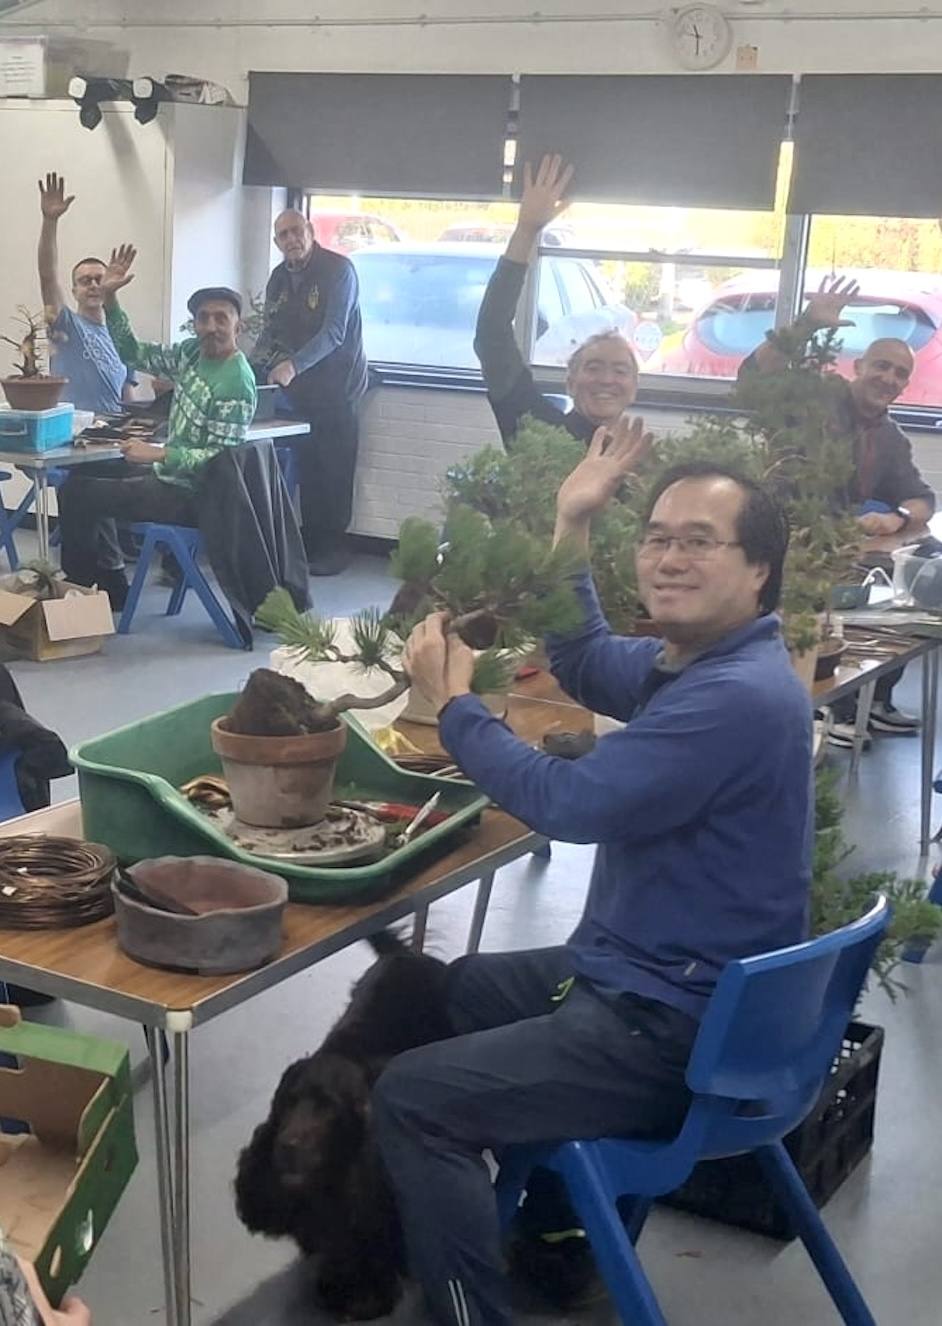
\includegraphics[angle=0,origin=c,width=1.0\textwidth]{2025_12/res/workshop-mep-members_2}
%%\centerline{\emph{Members gaining confidence during the session.}}
%%\end{minipage}
%%
%%\columnbreak
%
%
%
%
%\section*{Rooted in Success: A Masterclass in Soil and Nutrition}
%By [Your Name], Newsletter Editor
%
%Based on the TWBC Online Workshop by Andy Hardman
%
%During the quiet months of the pandemic, our club was privileged to host a deep-dive virtual workshop with \textbf{Andy Hardman}.
%For those who missed it—or those whose notes have gathered dust—this article reorganizes Andy's masterclass on the horticultural "engine" of bonsai: the substrate and the nutrients we fuel it with.
%
%As we approach the repotting season, we have also synthesized this with the \textbf{TWBC New & Existing Members Information Pack} (available in full on our Discord channel) to provide a comprehensive guide for every bench in the club.
%
%\subsection*{The Anatomy of the Root System}
%To understand soil, Andy insists we first understand the tree's physiology. When we look at a tree, we admire the \textit{nebari}(the surface roots), but the heavy lifting is done by millions of microscopic \textbf{root hairs}.
%
%Unlike the thick, woody transport roots, these hairs are incredibly delicate and short-lived. They do not grow "in" the soil so much as they cling "to" it. They require a physical surface to adhere to. Therefore, the goal of a bonsai soil is not just to "hold the tree up," but to provide the maximum possible surface area for these hairs to colonize.
%
%When we bare-root a tree during repotting, we are essentially stripping these hairs away. This is why our choice of substrate is so critical: if the soil is right, the tree recovers in weeks; if the soil is wrong, the tree may struggle for a year.
%
%\subsection*{The Physics of the Pot: Oxygen and Water}
%Andy's philosophy centers on a "particulate porous substrate." He identifies three non-negotiables for any mix:
%
%\begin{enumerate}
%\item \textbf{Aeration:} Roots need oxygen to perform the chemical processes required for growth.
%
%
%\item \textbf{Drainage:} Water must move through the pot to pull fresh oxygen behind it.
%
%
%\item \textbf{Water Retention:} The particles themselves must soak up enough moisture to keep the root hairs hydrated without drowning them.
%
%
%\end{enumerate}
%\subsubsection*{The "Two-Millimeter" Rule}
%A key takeaway from Andy's talk was the impact of \textbf{Surface Tension}. If soil particles are too small (dust or fine sand), the gaps between them are so narrow that water creates a "bridge" across the gap. This seals the soil, preventing gas exchange and suffocating the roots.
%
%Andy recommends a particle size of \textbf{$2\text{--}3\text{ mm}$}. This is the "sweet spot" where the gaps are large enough to break surface tension, allowing excess water to drain out and oxygen to rush in, while the particles remain small enough to maximize the surface area for root hairs.
%
%\subsection*{The Science of "CEC" (Cationic Exchange Capacity)}
%One of the more technical aspects Andy covered was \textbf{CEC}. Think of this as the soil's "magnetic" ability to hold onto food. Most nutrients, when dissolved in water, carry a slight electrical charge.
%
%Substrates with high CEC (like Akadama) act like a battery, "holding" the nutrients so they aren't immediately washed out the bottom of the pot. Substrates with zero CEC (like common horticultural grit) provide no nutritional storage. By choosing high-CEC materials, you create a more "efficient" root system where food is always available on the surface of the particles where the root hairs live.
%
%\subsection*{Evaluating the Substrates}
%Andy provided a "report card" for the most common materials:
%
%\begin{itemize}
%\item \textbf{Akadama:} The gold standard for many. It has excellent CEC, incredible texture, and holds water perfectly. However, it is a "partly baked" clay. Its weakness is the freeze-thaw cycle. If water inside an Akadama particle freezes, it expands ($V_{ice} \approx 1.09 \times V_{water}$), shattering the particle into dust.
%
%
%\item \textbf{Pumice & Lava:} These are Andy's "all-rounders." They are volcanic, incredibly hard, and will not break down in frost. They have medium-to-good CEC and provide the rough, jagged surface that encourages roots to split and ramify.
%
%
%\item \textbf{Horticultural Grit:} Andy is notoriously skeptical of grit. It is hard, but it has zero porosity and zero CEC. In a small bonsai pot, he views grit as "wasted space" that could be occupied by a functional, porous material.
%
%
%\item \textbf{Cat Litter:} A viable, budget-friendly alternative to Akadama, provided it is the "non-clumping" calcined molar clay variety. It is harder than Akadama but often has a smoother surface and lower CEC.
%
%
%\end{itemize}
%\subsection*{The Feeding Regime: N-P-K and Beyond}
%Once your soil is established, how do you fuel it? Andy broke down the "Macro-nutrients" that every member should recognize on a fertilizer label:
%
%\begin{itemize}
%\item \textbf{Nitrogen (N):} The engine of green growth and chlorophyll.
%
%
%\item \textbf{Phosphorus (P):} Strengthens the cambium, roots, and aids in flower/fruit production.
%
%
%\item \textbf{Potassium (K):} The "regulator" for the tree's internal systems and disease resistance.
%
%
%\end{itemize}
%\subsubsection*{Seasonal Strategy}
%Andy suggests shifting your N-P-K ratios based on the tree's annual cycle:
%
%\begin{enumerate}
%\item \textbf{Spring:} A higher Nitrogen ratio (e.g., $10\text{--}6\text{--}6$) helps trees in development put on mass and "charge their batteries."
%
%
%\item \textbf{Summer:} Switch to a balanced feed (e.g., $5\text{--}5\text{--}5$) as extension growth slows.
%
%
%\item \textbf{Late Summer/Autumn:} Drop the Nitrogen and increase Phosphorus and Potassium (e.g., $3\text{--}10\text{--}10$). This prepares the buds for next year and hardens the wood for winter.
%
%
%\end{enumerate}
%\subsubsection*{Organic vs. Chemical}
%Andy's stance is firm: \textbf{Go Organic.} Chemical fertilizers are salts. While they work fast, they can kill the beneficial microorganisms and mycorrhizal fungi that live in your soil. Organic pellets (like Bio-Gold or Naruko) rely on these bacteria to break them down, creating a healthy, living "micro-culture" inside the pot.
%
%\subsection*{TWBC Insights: From the Members' Pack}
%While Andy's talk provides the scientific foundation, our club's \textbf{New & Existing Members Information Pack} (available on Discord) provides practical local advice for our specific UK climate.
%
%\subsubsection*{The "John Innes" Alternative}
%While Andy leans toward a purely mineral mix (Lava/Pumice/Akadama), many club members have found success with a more traditional mix of \textbf{John Innes No. 3 and horticultural grit}. This is often more forgiving for those who cannot water twice a day in the heat of summer. However, the club echoes Andy's warning: organic compost \textit{will} break down over time. If you use this mix, expect to repot more frequently to prevent compaction and "sour" soil.
%
%\subsubsection*{Winter Care and "Tony U's" Concoction}
%The Members' Pack emphasizes that while native trees are hardy, the shallow nature of a bonsai pot leaves roots vulnerable. We recommend protection in a cold frame or unheated greenhouse during deep freezes.
%
%For those looking to clean their trees during the dormant season, the pack includes \textbf{Tony U's Winter Wash recipe}, a club favorite for tackling overwintering pests without harsh chemicals:
%
%\begin{itemize}
%\item $1\text{ liter}$ filtered water
%
%
%\item $1\text{ tbsp}$ Neem Oil
%
%
%\item $1\text{ tbsp}$ White Vinegar
%
%
%\item $1\text{ tsp}$ Washing-up liquid (as an emulsifier)
%
%
%\end{itemize}
%\textit{Note: Use a toothbrush to apply to the bark, but cover your moss first—the vinegar will kill it!}
%
%\subsection*{Final Thoughts}
%As Andy concluded in his workshop, "A healthy tree starts at the roots." Whether you choose the high-tech mineral approach of Akadama and Pumice or the classic John Innes mixes mentioned in our Discord news, the goal remains the same: balance.
%
%\textbf{Next Steps for Members:}
%
%\begin{itemize}
%\item Check the \textbf{Discord "News" channel} for the link to the full Information Pack.
%
%
%\item Start sifting your soils now—repotting season is just around the corner!
%
%
%\end{itemize}
%
%
%
%
%
%
%
%
%
%
%
%
%\section{Rooted in Success: A Masterclass in Soil and Nutrition}
%
%\textit{By [Your Name], Newsletter Editor}
%
%During the quiet months of the pandemic, our club was privileged to host a deep-dive virtual workshop with \textbf{Andy Hardman}. For those who missed it—or those whose notes have gathered dust—this article reorganizes Andy's masterclass on the horticultural "engine" of bonsai: the substrate and the nutrients we fuel it with.
%
%As we approach the repotting season, we have also synthesized this with the \textbf{New & Existing Members Information Pack} stored on our \textbf{Discord channel} (and linked among the bonsai news in this newsletter).
%
%\section{The Physiology of the Root System}
%
%To understand soil, Andy insists we first understand the tree's physiology. When we look at a tree, we admire the \textit{nebari} (the surface roots), but the heavy lifting is done by millions of microscopic \textbf{root hairs}.
%
%Unlike the thick, woody transport roots, these hairs are incredibly delicate and short-lived. They do not grow "in" the soil so much as they cling "to" it. They require a physical surface to adhere to. Therefore, the goal of a bonsai soil is not just to provide stability, but to provide the maximum possible surface area for these hairs to colonize.
%
%When we bare-root a tree during repotting, we are essentially stripping these hairs away. This is why our choice of substrate is so critical: if the soil is right, the tree recovers in weeks; if the soil is wrong, the tree may struggle for a year or more. A strong, vigorous tree starts at its roots. Without a strong network, the tree becomes weak and susceptible to pests and disease.
%
%\section{The Physics of the Pot: Oxygen and Water}
%
%Andy's philosophy centers on a \textit{particulate porous substrate}. He identifies three non-negotiables for any mix: \textbf{Aeration, Drainage, and Water Retention.}
%
%\subsection{The Two-Millimeter Rule} A key takeaway from Andy's talk was the impact of \textbf{Surface Tension}. If soil particles are too small (dust or fine sand), the gaps between them are so narrow that water creates a "bridge" across the gap. This seals the soil, preventing gas exchange and suffocating the roots.
%
%Andy recommends a particle size of: 2 mm≤Size≤3 mm
%
%This is the "sweet spot" where the gaps are large enough to break surface tension, allowing excess water to drain out and oxygen to rush in, while the particles remain small enough to maximize the surface area. Using larger particles, such as 5 mm or 6 mm, is acceptable for large trees in big boxes, but for refined bonsai, it wastes valuable pot vol_1.
%
%\subsection{CEC: Cationic Exchange Capacity} One of the more technical aspects Andy covered was \textbf{CEC}. Think of this as the soil's "magnetic" ability to hold onto food. Most nutrients, when dissolved in water, carry a slight electrical charge. Substrates with high CEC (like Akadama) act like a battery, "holding" the nutrients so they aren't immediately washed out. Substrates with zero CEC (like common horticultural grit) provide no nutritional storage.
%
%\section{Evaluating the Substrates}
%
%Andy provided a "report card" for the most common materials we use:
%
%\begin{itemize} \item \textbf{Akadama:} The gold standard for many. It has excellent CEC and holds water perfectly. However, it is a clay-based subsoil. Its weakness is the freeze-thaw cycle. If water inside an Akadama particle freezes, it expands (Vice​≈1.09×Vwater​), shattering the particle into dust. \item \textbf{Pumice & Lava:} These are Andy's "all-rounders." They are volcanic, incredibly hard, and will not break down in frost. They have a medium-to-good CEC and provide the rough, jagged surface that encourages roots to split and ramify. \item \textbf{Horticultural Grit:} Andy is notoriously skeptical of grit. It is hard, but it has zero porosity and zero CEC. In a small bonsai pot, he views grit as "wasted space." \item \textbf{Cat Litter:} A viable, budget-friendly alternative, provided it is the "non-clumping" molar clay variety. It is harder than Akadama but often has a smoother surface and lower CEC. \end{itemize}
%
%\section{The Feeding Regime: N-P-K and Beyond}
%
%Once your soil is established, how do you fuel it? Andy broke down the "Macro-nutrients":
%
%\begin{itemize} \item \textbf{Nitrogen (N):} Produces green growth, strong stems, and chlorophyll. \item \textbf{Phosphorus (P):} Helps roots and cambium cells; aids in flower and fruit production. \item \textbf{Potassium (K):} Helps the overall system function and disease resistance. \end{itemize}
%
%\subsection{Seasonal Strategy} Andy suggests shifting your N-P-K ratios based on the tree's annual cycle. In \textbf{Spring}, a higher Nitrogen ratio (e.g., 10:6:6) helps trees in development. By \textbf{Summer}, switch to a balanced feed (5:5:5). In \textbf{Late Summer/Autumn}, drop the Nitrogen and increase Phosphorus and Potassium (e.g., 3:10:10) to prepare the buds for next year.
%
%\subsection{Organic vs. Chemical} Andy's stance is firm: \textbf{Go Organic.} Chemical fertilizers are man-made salts. While they work fast, they can kill the beneficial bacteria and microorganisms in the soil. Organic pellets (like \textit{Bio-Gold, Green Dream,} or \textit{Naruko}) rely on these bacteria to break them down, creating a healthy, living "micro-culture" inside the pot.
%
%\section{TWBC Insights: From the Members' Pack}
%
%While Andy's talk provides the scientific foundation, our club's \textit{New & Existing Members Information Pack} (available on Discord) provides practical local advice.
%
%\subsection{The John Innes Alternative} While Andy leans toward a purely mineral mix, many club members have found success with a mix of \textbf{John Innes No. 3 and horticultural grit}. This is often more forgiving for those who cannot water twice a day. However, we must remember that organic compost contains dead plant material that \textit{will} break down and become compacted over time, reducing drainage.
%
%\subsection{Winter Care and "Tony U's" Concoction} Native trees are hardy, but bonsai in shallow pots need protection from frost in a greenhouse or cold frame. For those looking to apply a \textbf{Winter Wash} to deciduous trees, our own Tony U has a specialized recipe: \begin{itemize} \item 1 liter non-flavoured filtered water \item 1 tbsp Neem Oil \item 1 tbsp White Vinegar \item 1 tsp Washing-up liquid \end{itemize} \textit{Apply with a toothbrush, but ensure you cover your moss first, as the vinegar will kill it!} Alternatively, a diluted \textbf{Lime Sulfur} wash (ratio 20:1) is advised, taking care to cover the soil during application.
%
%\section{Summary} As Andy reminded us, the goal of our substrate is to create a "mini micro-culture" where mycorrhizae and healthy bacteria thrive. Whether you follow the mineral-heavy path of Akadama and Pumice or the more traditional John Innes mixes, the health of your tree is a direct reflection of the environment you create beneath the soil line.
%
%For further details, please consult the full \textbf{Information Pack} on the TWBC Discord.
%
%
